\chapter{Project plan}
\section{Current progress}
At the time of writing, a simple minimal web application has been set up using React and TypeScript. It supports derivations for Curry types and the Lambda Calculus \textit{without} bracketing conventions, i.e. $\lambda$-terms and types must be fully bracketed. Screenshots of the web application in use can be seen in \Cref{demo:incomplete} and \Cref{demo:complete}.

\begin{figure}[!htbp]
    \centering
    \begin{minipage}[t]{0.5\textwidth}
        \centering
        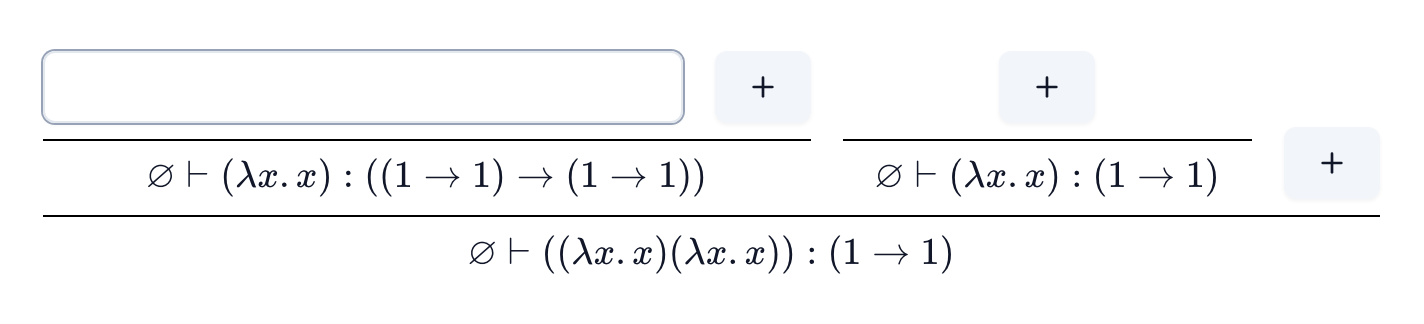
\includegraphics[width=\textwidth]{project/demo-incomplete.png}
        \caption{An incomplete derivation tree}
        \label{demo:incomplete}
    \end{minipage}\hfill
    \begin{minipage}[t]{0.5\textwidth}
        \centering
        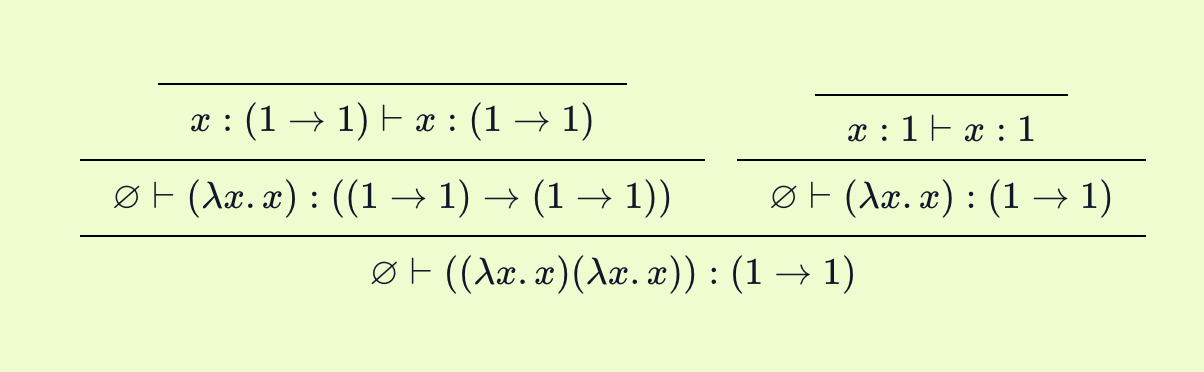
\includegraphics[width=\textwidth]{project/demo-complete.png}
        \caption{A complete derivation tree}
        \label{demo:complete}
    \end{minipage}
\end{figure}

Users input what they want to prove for each node of the tree in freeform text, with syntax half-inspired by Haskell and half-inspired by \LaTeX{}. For instance, \texttt{\textbackslash empty |- ((\textbackslash x.x)(\textbackslash x.x)): (1 -> 1)} gives the conclusions of \Cref{demo:incomplete} and \Cref{demo:complete}.

When the user inputs a well-formed conclusion for a node, a new blank text input appears as a premise, as in the leftmost subtree of \Cref{demo:incomplete}. At each level of the derivation tree is a button allowing users to add more blank inputs, and therefore more subtrees to the derivation. The buttons are hidden only when the user has built a fully correct and complete derivation tree. This ensures users are given minimal hints---hiding the button on a certain level when the correct number of subtrees is built would be a hint, for example.

\section{Next steps and extensions}
After an initial meeting with Prof. van Bakel, it was agreed that the immediate next step would be to define the syntax and semantics for inference rules, starting from those applicable to the Curry type assignment system for the Lambda Calculus. This would allow us to replace the current hard-coded verifier rules for the Lambda Calculus by defining the inference rules in the web application and compiling these rules into a verifier program. We may then extend the language for defining inference rules to other systems, such as the Gentzen-style sequent calculus and Milner's \textsc{ML}.

There are certain tasks that are important for a pleasant user experience. They are, in various levels of significance:
\begin{itemize}
    \item Extending the parsers to adopt the bracketing conventions outlined in \Cref{background}, so that users can drop brackets as they would when writing derivations by hand. Unit tests are be needed to verify the correctness of the EBNF syntaxes proposed in \Cref{background} and the behaviour of the parsers.
    \item Extending the input syntax to support multiple ways of inputting the same symbols
    \item Investigating alternatives for inputting the statements, such as
    \begin{itemize}
        \item Drag-and-drop blocks
        \item Structured text input, i.e. instead of one big text box, we can split it into multiple smaller text boxes depending on the syntax, e.g. \fbox{\rule{0.5in}{0pt}\rule{0pt}{4pt}} $\vdash$ \fbox{\rule{0.25in}{0pt}\rule{0pt}{4pt}} $:$ \fbox{\rule{0.25in}{0pt}\rule{0pt}{4pt}}
        \item Separating the text inputs from the nodes, so that users unfamiliar with the syntax can see the \LaTeX{} update in real time and adjust their input accordingly
    \end{itemize}
\end{itemize}

In addition to the core functionality of building derivation trees, we can explore extensions such as:
\begin{itemize}
    \item Supporting \LaTeX{} export of the derivation trees and proofs, to reduce the lecturers' workload for generating official mark schemes of new exercise problems, coursework, and exams, as well as allowing students to submit exercises in \LaTeX{} with ease
    \item Allowing users to save and load (possibly incomplete) derivations e.g. by writing and reading from a local file, so that users can complete large derivations in multiple sittings or modify existing derivations without having to rebuild them from scratch
    \item Gamifying the tool by e.g. providing a pre-defined set of exercise problems, similar to the Incredible Proof Machine \cite{incredibleproofmachine, breitner:2016}
    \item Rewriting Pandora with more intuitive user interactions
\end{itemize}

\section{Expected timeline}
The main coding parts are expected to be completed by the end of spring term. We expect progress to be mostly linear with respect to time spent as the bulk of setting up frameworks and libraries are already done. While further discussion with Prof. van Bakel is needed to fully define the scope of the project, we should be able to implement the core functionality and some extensions by the end of March.

Most of April would ideally be spent on coding extensions and getting started with the final report. The final report is expected to be done by the end of May, after which the main focus would be the final presentation and other deliverables.
